\documentclass{szzclass}

\title{Abstraktní datový typ, jeho specifikace a implementace. Zásobník, fronta, pole, seznam, tabulka, množina. Implementace pomocí pole, spojových struktur a stromů.}
\author{Jakub Rathouský}

\begin{document}
\maketitle
\tableofcontents
\newpage

\section{Abstraktní datový typ}
Abstraktní datové typy (ADT) definují množinu hodnot a operací nezávisle na konkrétní implementaci.
\subsection{Specifikace}
ADT může být formálně specifikován signaturou operací a množinou axiomů.
\begin{itemize}
    \item axiomy jsou ekvivalence mezi výrazy, každý výraz reprezentuje stav
    \item výrazy jsou složené z operací a proměnných
    \item axiomy mohou být použity pro zjednodušení komplexnějších výrazů
\end{itemize}
\begin{figure}[h!]
    \centering
    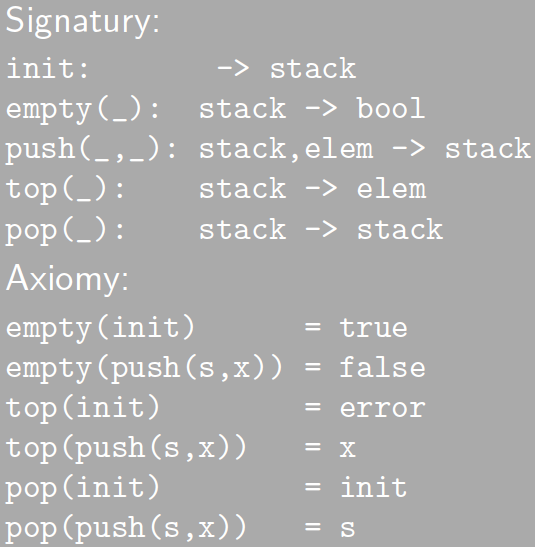
\includegraphics[width=0.5\textwidth]{topics/bi-spol-22/images/ADT_signature_axiom.png}
    \caption{Ukázka popisu signatury a axiomů zásobníku}
    \label{ADT_SIGNATURE_AXIOM}
\end{figure}
\subsection{Implementace}
Některé programovací jazyky (například Clear) dovolují formální specifikace ADT. Imperativní (a OOP) jazyky
vyžadují explicitní implementaci ADT. V C++ je doporučeno implementovat ADT generickými třídami:
\begin{itemize}
    \item typ prvku je generickým parametrem šablony třídy
    \item operace init je implementována konstruktorem
    \item implementace obvykle používá dynamicky alokovanou paměť, proto je často vyžadován i destruktor, kopírující konstruktor a přetížený operátor =
    \item když je signatura operace ADT, $\dots \rightarrow elem$ je doporučená implementace const metodou vracející T
    \item když je signatura operace ADT, $\dots \rightarrow ADT$ je doporuřeno implementace metodou modifikující objekt
\end{itemize}
\section{Struktury}
\subsection{Zásobník}
\subsubsection{Implementace}
\begin{itemize}
    \item pole pevné délky, kapacita je omezena už při kompilaci
    \item dynamicky alokované pole, velikost pole je dána parametrem konstruktoru
    \item dynamicky alokované pole, velikost pole se mění
    \item spojový seznam
\end{itemize}
Časová složitost je konstantní jak pro metodu push, tak pro pop. Jen pro dynamicky alokované pole s měnící se velikostí se liší:
\begin{itemize}
    \item když je velikost pole měněna při každém push, složitost push je lineární
    \item když je velikost pole zdvojnásobována (nebo víc), je režije amortizována a push by byl průměrně konstantní
\end{itemize}
\subsection{Fronta}
\subsubsection{Popis}
Fronta je sekvenční kontejner organizovaný FIFO způsobem. Způsoby implementace:
\subsubsection{Implementace}
\begin{itemize}
    \item polé pevné délky, kapacita (maximální počet prvků ve frontě) je omezena už při kompilaci
    \item dynamicky alokované pole, velikost pole je dána parametrem konstruktoru, opět omezená paměť
    \item dynamicky alokované pole, velikost je měněna vždy, když je potřeba
    \item spojový seznam (jednosměrně zřetězen)
\end{itemize}
Časová složitost je konstatní (pro push i pop). Jediná výjimka je dynamicky alokované pole s měnící se velikostí, zde
může být složinost až O(n), ale průměrná může být stále konstatní při exponenciálním nárustu velikosti.

\subsection{Pole}
\subsubsection{Popis}
Pole je datový kontejner, který organizuje prvky v n-dimenzionálním prostoru:
\begin{itemize}
    \item náhodný přístup k prvkům s konstantní časovou složitostí
    \item prvek je identifikován n-ticí indexů (celých čísel)
\end{itemize}
\subsubsection{Implementace - jednodimenzionální pole}
array[$l_1 \dots h_1$]
\newline
Prvky uloženy v kontinuálním paměťovém bloku, velikost bloku: ($(h_1 - l_1 + 1) * sizeof(T)$). Funkce zajišťující přístup k prvku (mapovací funkce map(i))
je ofset prvku od počátečního bloku.
\newline
Jednodimenzionální pole má jednoduchou mapovací funkci: $map(i) = (i - l_1)$. Protože pole v C/C++, Javě, C\#... má vždy $ l_1 = 0 $, tak je mapovací
funkce ještě jednodušší = $map(i) = i$
\subsubsection{Implementace - multidimenzionální pole}
array[$l_1 \dots h_1,l_2 \dots h_2,\dots,l_n \dots h_n$]
\newline
Jediný kontinuální blok, serializace "po řádcích" (nejpravější index roste nejrychleji).
Jediný kontinuální blok, serializace "po sloupcích" (nejlevější index roste nejrychleji).
Přístupové vektory (lliffe-ho vektory).
\begin{figure}[h!]
    \centering
    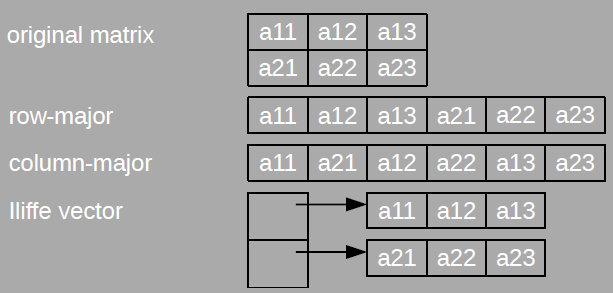
\includegraphics[width=0.4\textwidth]{topics/bi-spol-22/images/multidimensionalArray.png}
    \caption{Příklad interní reprezentace pole}
\end{figure}

\subsection{Seznam}
\subsubsection{Popis}
Seznam je datová struktura, která poskytuje operace insert, remove a read. Operace jsou určeny pozicí v seznamu. Pozice může být měněna.
\subsubsection{Implementace}
Požadujeme konstantní časovou složitost pro všechny operace. Proto nemůže být použito pole. Struktura zřetězeného seznamu dovoluje provádění vložení
a rušení s konstantní časovou složitostí. Obousměrně zřetězený seznam je použit pro dosažení konstantního času i pro operaci \textit{o jedno zpět(toPrev)}.
Pro operaci \textit{na konec (toEnd)} je použit ukazatel na konec pole.

\subsection{Množina}
\subsubsection{Popis}
Kontejner, který obsahuje prvky typu T, bez duplikátů. Základní interface:
\begin{itemize}
    \item vložení prvku (insert)
    \item odstranění prvku (remove)
    \item test přítomnosti prvku
\end{itemize}
\subsubsection{Implementace}
\begin{itemize}
    \item indikátorový (charakteristický) vektor
    \item pole (neseřazené)
    \item pole (seřazené)
    \item spojový seznam (jednosměrný, neseřazený)
    \item spojový seznam (jednosměrný, seřazený)
    \item binární vyhledávací strom
    \item rozptylovací funkce (hash table)
\end{itemize}
\subsubsection{Implementace - indikátorový vektor}
Funkce, který má hodnotu 0 pro prvky nepatřící do množiny 1 pro prvky v množině obsažené. \newline
Když je universum konečné a dostatečně malé, může být funkce implementována jako vektor. \newline
Vektor obsahuje hodnoty typu bool nebo je to bitové pole. \newline
Implementace je rychlá:
\begin{itemize}
    \item insert(x) - O(1)
    \item del(x) - O(1)
    \item isSet(x) - O(1)
\end{itemize}
Jiné operace:
\begin{itemize}
    \item průnik - vytvoření nové množiny, procházení jedné množiny (O(n)) a testování existence v druhé (O(1)) = O(n) celkem
    \item sjednocení - vytvoření nove množiny, procházení prvků první množiny (O(n)), vkládání jejich prvků (to samé i pro druhou množinu) = O(n + n) = O(n)
    \item porovnání - porovnávají se všechny prvky obou množin - O(n)
\end{itemize}
\subsubsection{Implementace - neseřazené pole}
Neseřazené prvky jsou umístěny v poli, které je dynamicky alokované a jeho velikost se mění. Třída musí mít přehled o velikosti pole
a o počtu prvků v množině.
\begin{itemize}
    \item insert(x) - nový prvek se umístí na konec pole (O(1)). To může způsobit duplicitu. Proto se musí nejdříve otestovat projitím pole (O(n)) = O(n)
    \item del(x) - prochází se pole (O(n)) a když je prvek nalezen, nahradí se posledním prvkem pole (O(1)) = O(n)
    \item isSet(x) - hledá se v poli (O(n)) = O(n)
\end{itemize}
Jiné operace:
\begin{itemize}
    \item průnik - vytvoření nové množiny, procházení prvků první množiny (O(n)) a test přítomnosti v druhé množině (O(m)) = O(n*m)
    \item sjednocení - vytvoření nové množiny, procházení prvků první množiny a vkládání jejích prvků (O(n)). Pak procházení druhé množiny + kontrola existence (O(n*m)) = O(n*m)
    \item porovnání - porovnává se obsah polí (kvadratický algoritmus): O(n*m)
\end{itemize}
\subsubsection{Implementace - seřazené pole}
Seřazené prvky jsou umístěny v poli, které je dynamicky alokované a jeho velikost se mění. Třída musí mít přehled o velikosti pole
a o počtu prvků v množině.
\begin{itemize}
    \item insert(x) - místo pro vložení se najde binárním hledáním (O(log n)). Pak ale prvky za tímto místem musí být odsunuty pravo (O(n)) = O(n)
    \item del(x) - prvek se najde binárně (O(log n)), ale opět se musí posunout (O(n)) po vymazání = O(n)
    \item isSet(x) - v poli se hledá binárně (O(log n)) = O(log n)
\end{itemize}
Jiné operace:
\begin{itemize}
    \item průnik - vytvoří se nová množina, obě se projdou simultánně. Vloží se vždy jeden ze stejných prvků = O(max(n, m))
    \item sjednocení - vytvoření nové množiny, obě množiny se procházejí sumultánně. Vloží se všechny prvky (stejné jen jednou) = O(max(n, m))
    \item porovnání - porovnají se pole (lineární algoritmus) = O(max(n, m))
\end{itemize}
\subsubsection{Implementace - spojový seznam}
Neseřazený spojový seznam: implementace je stejná jako u neseřazeného pole.\newline
Seřazený spojový seznam: implementace vložení/odstranění/test přítomnosti je stená jako u neseřazeného pole. Sjednocení/průnik/porovnání mohou být
implementovány lépe - jako u seřazeného pole.\newline
Implementace spojovým seznamem má větší režii na paměť než seřazené pole.


\subsection{Tabulka (Mapa, Slovník)}
\subsubsection{Popis}
Kontejner, který obsahuje dvojice klíč-hodnota. Klíče jsou unikátní. Základní interface:
\begin{itemize}
    \item \textit{init: -> Map},
    \item vložení klíče s hodnotou (insert) \textit{ins(\_,\_,\_): Key, Val, Map -> Map},
    \item odstranění klíče s hodnotou (remove) \textit{del(\_,\_): Key, Map -> Map},
    \item test přítomnosti klíče \textit{isSet(\_,\_): Key, Map -> bool},
    \item výběr hodnoty podle klíče \textit{read(\_,\_): Key, Map -> Val}.
\end{itemize}

Lze iterovat přes dvojice klíč-hodnota nebo pouze přes klíče nebo pouze přes hodnoty.

Mapy a množiny jsou podobné. Množinu můžeme považovat
za speciální případ mapy, kde hodnoty jsou typu \textit{bool}.

\subsubsection{Implementace}
\begin{itemize}
    \item pole - přímý přístup (klíče jsou indexy v poli)
    \item pole (neseřazené)
    \item pole (seřazené)
    \item spojový seznam (jednosměrný, neseřazený)
    \item spojový seznam (jednosměrný, seřazený)
    \item binární vyhledávací strom
    \item rozptylovací funkce (hash table)
\end{itemize}
\subsubsection{Implementace - pole - přímý přístup}
Klíče mohou být pouze celá čísla z intervalu 0 až maximální délka pole.
Nepřítomnost prvku musí být určena speciální hodnotou (například NULL).
Implementace je rychlá:
\begin{itemize}
    \item insert(k, v) - O(1)
    \item del(k) - O(1)
    \item isSet(k) - O(1)
    \item read(k) - O(1)
\end{itemize}

\subsubsection{Implementace - neseřazené pole}
Pole obsahuje neseřazené páry klíč-hodnota. Nové prvky jsou přidávány na konec pole.
Při hledání klíče se musí projít celé pole.
\begin{itemize}
    \item insert(k, v) - nový prvek se umístí na konec pole (O(1)). To může způsobit duplicitu. Proto se musí nejdříve otestovat projitím pole (O(n)) = O(n)
    \item del(k) - prochází se pole (O(n)) a když je prvek nalezen, nahradí se posledním prvkem pole (O(1)) = O(n)
    \item isSet(k) - hledá se v poli (O(n)) = O(n)
    \item read(k) - hledá se v poli (O(n)) = O(n)
\end{itemize}
Jiné operace:

\subsubsection{Implementace - seřazené pole}
Pole obsahuje seřazené páry klíč-hodnota.
Při hledání klíče se využije binární vyhledávání.
\begin{itemize}
    \item insert(k,v) - místo pro vložení se najde binárním hledáním (O(log n)). Pak ale prvky za tímto místem musí být odsunuty pravo (O(n)) = O(n)
    \item del(k) - prvek se najde binárně (O(log n)), ale opět se musí posunout (O(n)) po vymazání = O(n)
    \item isSet(k) - v poli se hledá binárně (O(log n)) = O(log n)
    \item read(k) - v poli se hledá binárně (O(log n)) = O(log n)
\end{itemize}

\end{document}
